\subsection{Sensores en General}

\par
Un sensor es un dispositivo capaz de detectar magnitudes físicas o químicas, llamadas variables de instrumentación, y transformarlas en variables eléctricas.\cite{sensores-wiki}

\begin{itemize}
	\item Las variables de instrumentación pueden ser, por ejemplo: temperatura, intensidad lumínica, distancia, aceleración, inclinación, desplazamiento, presión, fuerza, torsión, humedad, movimiento, pH, etc.\cite{sensores-wiki}
	
	\item Una variable eléctrica puede ser una resistencia eléctrica (como en una RTD), una capacidad eléctrica (como en un sensor de humedad o un sensor capacitivo), una tensión eléctrica (como en un termopar), una corriente eléctrica (como en un fototransistor), etc.\cite{sensores-wiki}
\end{itemize}

\par \noindent
Los sensores se pueden clasificar en función de los datos de salida en: digitales y analógicos\cite{sensores-arduino}.

\subsubsection{Características de los Sensores}

\par \noindent
Las características son\cite{sensores-wiki}:

\begin{itemize}
	
	\item Rango de medida: dominio en la magnitud medida en el que puede aplicarse el sensor.
	
	\item Precisión: es el error de medida máximo esperado.
	
	\item Offset o desviación de cero:  valor de la variable de salida cuando la variable de entrada es nula. Si el rango de medida no llega a valores nulos de la variable de entrada, habitualmente se establece otro punto de referencia para definir el offset.
	
	\item Linealidad o correlación lineal.
	
	\item Sensibilidad de un sensor: suponiendo que es de entrada a salida y la variación de la magnitud de entrada.
	
	\item Resolución: mínima variación de la magnitud de entrada que puede detectarse a la salida.
	
	\item Rapidez de respuesta: puede ser un tiempo fijo o depender de cuánto varíe la magnitud a medir. Depende de la capacidad del sistema para seguir las variaciones de la magnitud de entrada.
	
	\item Derivas: son otras magnitudes, aparte de la medida como magnitud de entrada, que influyen en la variable de salida. Por ejemplo, pueden ser condiciones ambientales, como la humedad, la temperatura u otras como el envejecimiento (oxidación, desgaste, etc.) del sensor.
	
	\item Repetitividad: error esperado al repetir varias veces la misma medida.\cite{sensores-wiki}
	
\end{itemize}

\par \noindent
Debido a que solamente la magnitud física importante para el proyecto es la temperatura. Se tomarón en cuenta los posibles candidatos para utilizar como sensor de temperatura en el dispositivo, pero primero se presentará la definición formal de temperatura y los diversos termómetros existentes

\subsubsection{Termómetros}

\par 
El termómetro es un instrumento de medición de temperatura. Desde su invención ha evolucionado mucho, principalmente a partir del desarrollo de los termómetros electrónicos digitales. La manera como un termómetro determina la temperatura depende del tipo de termómetro que sea\cite{termometro}. 

\par \noindent
Inicialmente se fabricaron aprovechando el fenómeno de la dilatación, por lo que se prefería el uso de materiales con elevado coeficiente de dilatación, de modo que, al aumentar la temperatura, su estiramiento era fácilmente visible. La sustancia que se utilizaba más frecuentemente en este tipo de termómetros ha sido el mercurio, encerrado en un tubo de vidrio que incorporaba una escala graduada, pero también alcoholes coloreados en termómetros grandes\cite{termometro}.

\begin{figure}[H]
	\centering
	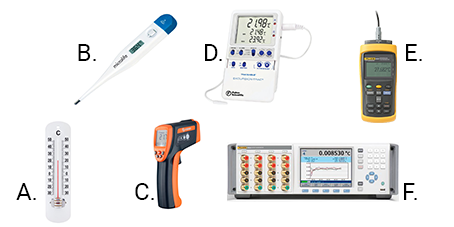
\includegraphics[width=\textwidth]{termometro1.png}
	\caption{Ejemplos de diferentes tipos de termómetros}
\end{figure}

\subsubsection{Escalas de temperatura}

\par 
La escala más usada en la mayoría de los países del mundo es la Celsius (\textdegree{}C) en honor a Anders Celsius (1701-1744) que se llamó centígrado hasta 1948. En esta escala, el cero (0 \textdegree{}C) y los cien (100 \textdegree{}C) grados corresponden respectivamente a los puntos de congelación y de ebullición del agua, ambos a la presión de 1 atmósfera.\cite{termometro}

\par \noindent 
Otras escalas termométricas son:\cite{termometro}

\begin{itemize}
	
	\item Fahrenheit (\textdegree{}F) 
	
	Propuesta por Daniel Gabriel Fahrenheit en la revista Philosophical Transactions (Londres, 33, 78, 1724). El grado Fahrenheit es la unidad de temperatura en el sistema anglosajón de unidades, utilizado principalmente en Estados Unidos.
	
	\item Kelvin (K) o temperatura absoluta: 
	
	Es la escala de temperatura del Sistema Internacional de Unidades. Aunque la magnitud de una unidad Kelvin (K) coincide con un grado Celsius (\textdegree{}C), el cero se ha fijado en el cero absoluto a -273,15 \textdegree{}C y es inalcanzable según el tercer principio de la termodinámica.
\end{itemize}

\subsubsection{Tipos de termómetros}

\begin{itemize}
	\item Termómetro de mercurio: es un tubo de vidrio sellado que contiene mercurio, cuyo volumen cambia con la temperatura de manera uniforme. Este cambio de volumen se aprecia en una escala graduada. El termómetro de mercurio fue inventado por Gabriel Fahrenheit en el año 1714. En la actualidad este tipo de termómetro ya no se fabrica\cite{termometro} Ver figura 1.15 (A)
	
	\item Pirómetros:  termómetros para altas temperaturas, se utilizan en fundiciones, fábricas de vidrio, hornos para cocción de cerámica, etc.\cite{termometro} Existen varios tipos según su principio de funcionamiento:
	
	\begin{itemize}
		
		\item Pirómetro óptico: se basan en la ley de Wien de distribución de la radiación térmica, según la cual, el color de la radiación varía con la temperatura. El color de la radiación de la superficie a medir se compara con el color emitido por un filamento que se ajusta con un reóstato calibrado. Se utilizan para medir temperaturas elevadas, desde 700 °C hasta 3.200 °C, a las cuales se irradia suficiente energía en el espectro visible para permitir la medición óptica. Ver figura 1.15 (B)
		
	\end{itemize}
	
	\item Termómetro de lámina bimetálica: formado por dos láminas de metales de coeficientes de dilatación muy distintos y arrollados dejando el coeficiente más alto en el interior. Se utiliza sobre todo como sensor de temperatura en el termohigrógrafo.
	
	\begin{figure}[H]
		\centering
		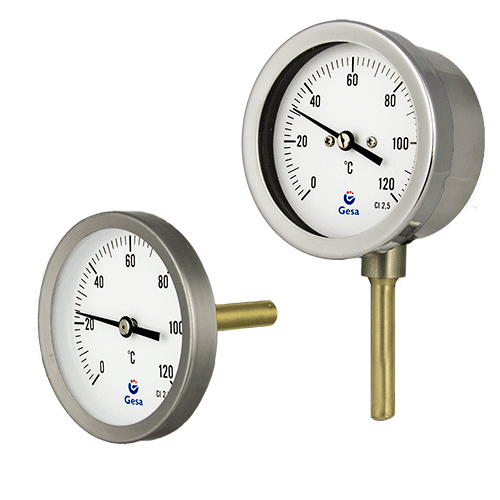
\includegraphics[width=5cm, height=5cm]{termometro2.png}
		\caption{Ejemplo de termómetro de lámina bimetálica}
	\end{figure}
	
	\item Termómetro de gas: pueden ser a presión constante o a volumen constante. Este tipo de termómetros son muy exactos y generalmente son utilizados para la calibración de otros termómetros.
	
	\begin{figure}[H]
		\centering
		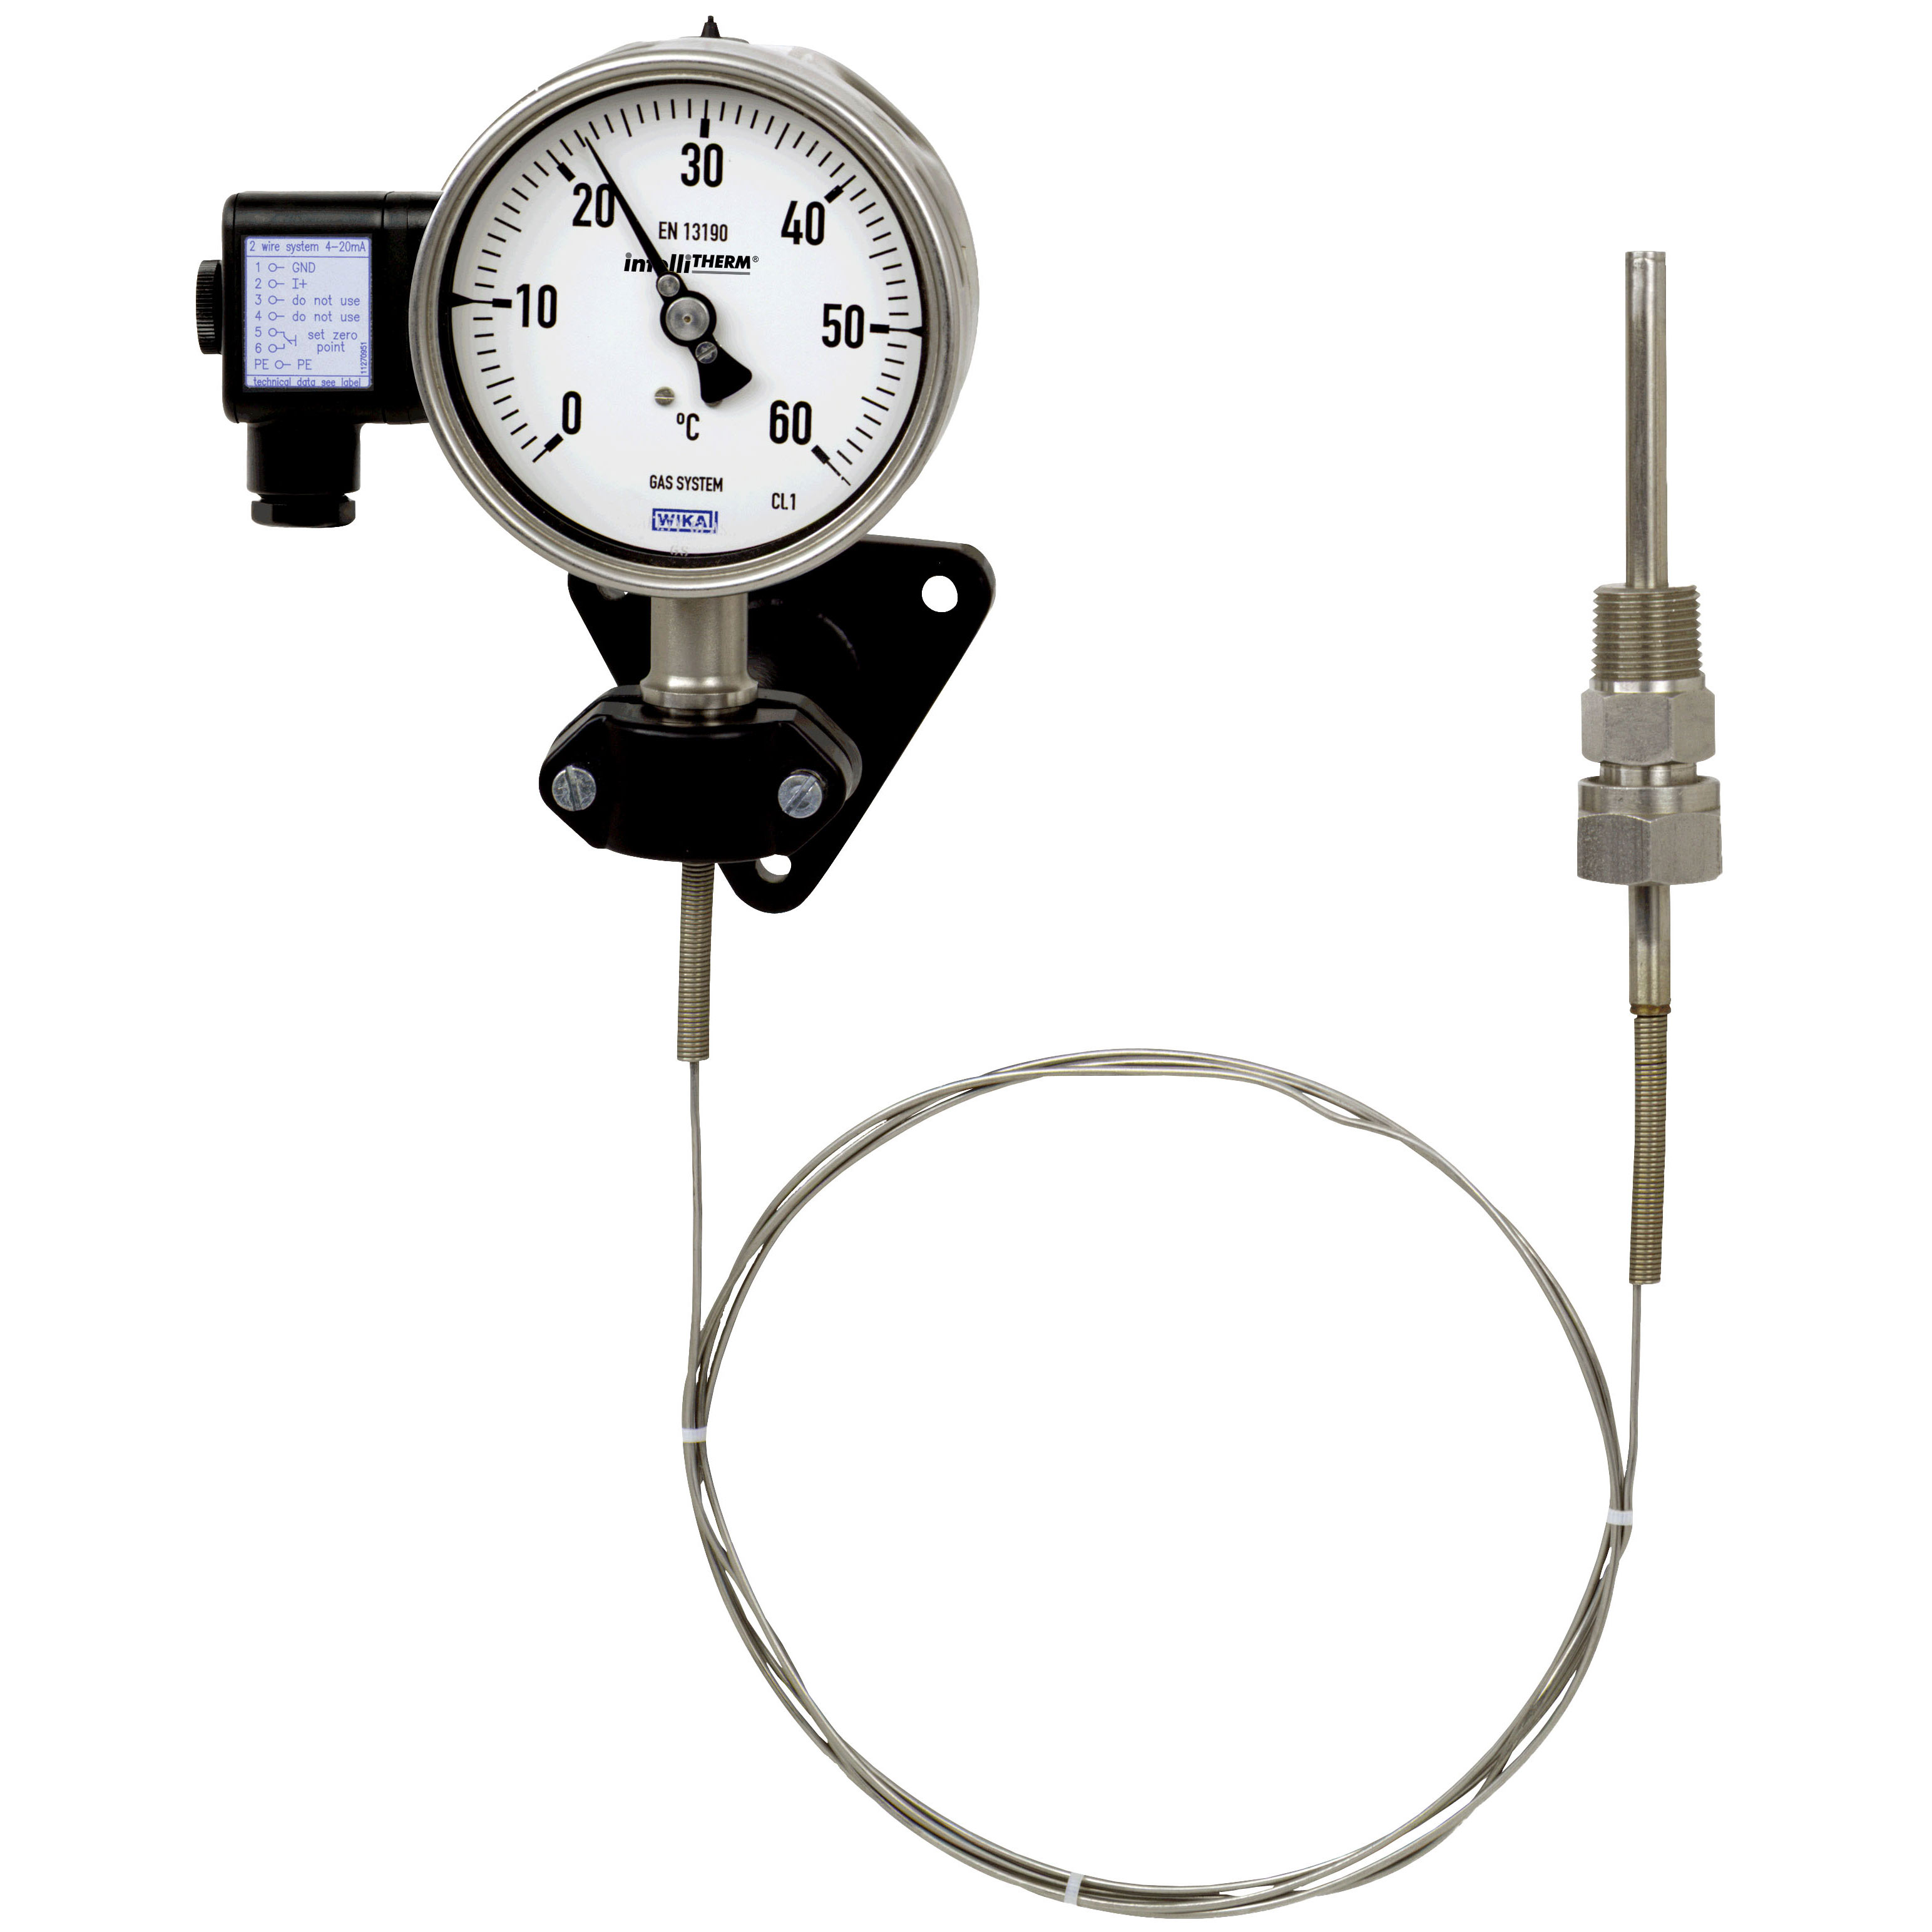
\includegraphics[width=4cm, height=4cm]{termometro3.jpg}
		\caption{Ejemplo de termómetro de gas}
	\end{figure}
	
	\item Termómetros digitales: son aquellos que, valiéndose de dispositivos transductores, utilizan luego circuitos electrónicos para convertir en números las pequeñas variaciones de tensión obtenidas, mostrando finalmente la temperatura en un visualizador. Una de sus principales ventajas es que por no utilizar mercurio no contaminan el medio ambiente cuando son desechados. Los dispositivos visualizadores pueden ser:
	
	\begin{itemize}
		
		\item Resistencia de platino: consiste en un alambre de algún metal de platino cuya resistencia eléctrica cambia cuando varía la temperatura. Van conectados a un termómetro digital como en la figura 1.15 (D, E y F)
		
		\item Termopar: También conocido como termocupla es un dispositivo utilizado para medir temperaturas basado en la fuerza electromotriz que se genera al calentar la soldadura de dos metales distintos. Van conectados a un termómetro digital como en la figura 1.15 (D y E)
		
		\item Termistor:  es un dispositivo que varía su resistencia eléctrica en función de la temperatura. Algunos termómetros hacen uso de circuitos integrados que contienen un termistor, como el LM35. Van conectados a un termómetro digital como en la figura 1.15 (D y E)
		
	\end{itemize}
	
	\item Termómetros clínicos: son los utilizados para medir la temperatura corporal. Los hay tradicionales de mercurio y digitales, teniendo estos últimos algunas ventajas adicionales como su fácil lectura, respuesta rápida, memoria y en algunos modelos alarma vibrante. Ver figura 1.15 (B)
	
	\item Termógrafo: El termógrafo es un termómetro acoplado a un dispositivo capaz de registrar, gráfica o digitalmente, la temperatura medida en forma continua o a intervalos de tiempo determinado. En la figura 1.15 (F) las mediciones van acompañadas de una gráfica.
	
\end{itemize}

\par \noindent
Dejado claro el concepto de termómetro y sus tipos, se procedió a investigar los sensores de temperatura que se pueden encontrar en la plataforma Arduino.

\subsubsection{Sensores de Temperatura}	

\begin{itemize}
	\item DS18B20: El termómetro digital DS18B20 proporciona de 9 bits a 12 bits.
	Mediciones de temperatura en grados Celsius y tiene una función de alarma no volátil programable por el usuario. El DS18B20 se comunica a través de un Bus de 1 cable que por definición requiere solo una línea de datos (y tierra) para la comunicación con un microprocesador central. Además, el DS18B20 puede obtener potencia directamente desde la línea de datos, eliminando la necesidad de una fuente de alimentación externa\cite{ds18b20}.
	
	\begin{figure}[H]
		\centering
		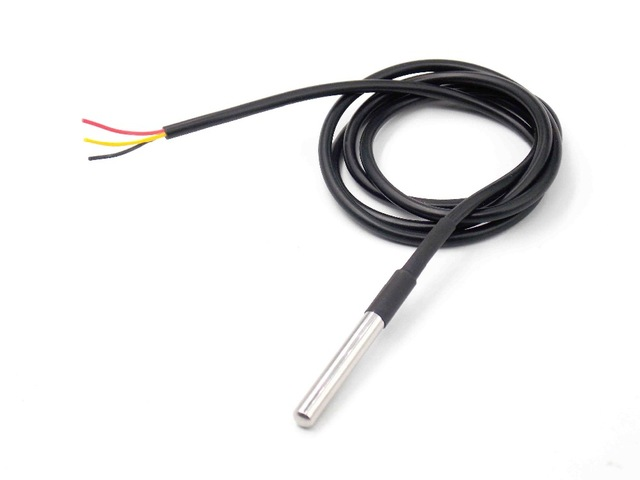
\includegraphics[width=0.5\textwidth]{sensores1.jpg}
		\caption{Sensor DS18B20 estilo sonda}
	\end{figure}
	
	\par \noindent
	Mide las temperaturas de -55 ° C a 125 ° C, ± 0.5 ° C de precisión entre -10 ° C a + 85 ° C y resolución programable de 9 a 12 bits.
	
	\par \noindent
	Las aplicaciones que pueden beneficiarse de esta característica incluyen
	controles ambientales, monitoreo de temperatura
	sistemas dentro de edificios, equipos o maquinaria, y
	sistemas de monitoreo y control de procesos\cite{ds18b20}. 
	
	\item DHT11: El sensor digital de temperatura y humedad DHT11 es un sensor compuesto que contiene una
	señal digital de salida de la temperatura y la humedad. Aplicación de módulos digitales dedicados
	tecnología de recolección y la tecnología de detección de temperatura y humedad, para asegurar que
	el producto tiene una alta fiabilidad y una excelente estabilidad a largo plazo. El sensor incluye un sentido resistivo
	de componentes húmedos y dispositivos de medición de temperatura NTC, y conectado con un
	microcontrolador de alto rendimiento de 8 bits\cite{dht11}.
	
	\begin{figure}[H]
		\centering
		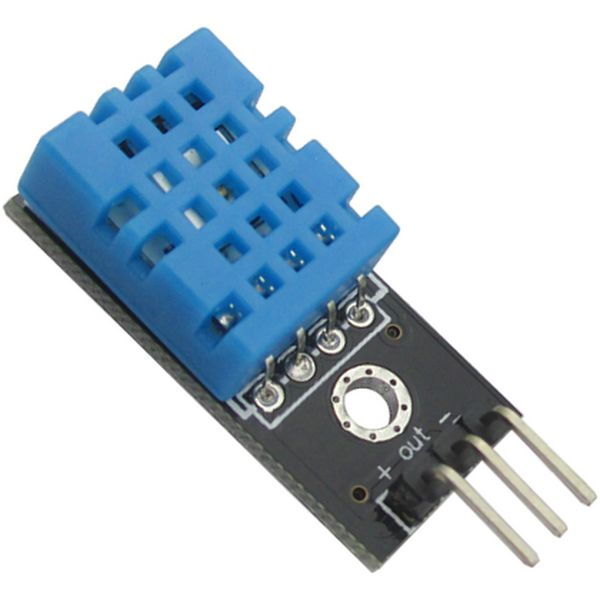
\includegraphics[width=0.25\textwidth]{sensores2.jpg}
		\caption{Sensor DHT11 en placa}
	\end{figure}
	
	\par \noindent
	Mide temperaturas de 0 ° C a 50 ° C con una precisión de ±2 ° C en 25 ° C y una resolución no programable de 16 bits.
	
	\par \noindent
	Las aplicaciones de este sensor son principalmente para mediciones de humedad y temperatura relativa. Donde se requiere obtener valores en ambas magnitudes y no tanta precisión de una magnitud en particular\cite{dht11}. 
	
\end{itemize}

\par \noindent
Luego de haber realizado la investigación sobre las diversas tecnologías existentes que podrían ser utilizadas en la elaboración de del arquetipo, se debió tener en consideración el lugar en el que fueron colocados los componentes, es por ellos que se toma en consideración la impresión 3D, la cual permite crear modelos físicos a partir de un modelo realizado por computadora. A continuación, se tratará más a fondo la impresión 3D.

